\documentclass[12pt, twoside, a4paper]{article}

%-------------------------------------------
% Margin settings
\usepackage[margin=2cm]{geometry}

%-------------------------------------------
% To insert the cover page
\usepackage{tikz}

%-------------------------------------------
% General packages
\usepackage[utf8]{inputenc}
\usepackage[brazil]{babel}
\usepackage[T1]{fontenc}
\usepackage{float}
\usepackage{graphicx}

%-------------------------------------------
% Hyper references
\usepackage{hyperref}
\hypersetup{
  colorlinks=true,
  linkcolor=black,
  citecolor=black,
  urlcolor=blue
}

%-------------------------------------------
% Customize fonts
\usepackage{bookman}
\usepackage{lmodern}

%-------------------------------------------
% Customize footer and headers
\usepackage{fancyhdr}
\pagestyle{fancy}
\lhead{VIII Encontro dos Alunos}
\chead{}
\rhead{21 a 23 de novembro, 2018}
\fancyfoot{}
\fancyfoot[LE,RO]{\thepage}
\renewcommand{\headrulewidth}{0.4pt}
\renewcommand{\footrulewidth}{0.0pt}

%-------------------------------------------
% Customize section's title
\usepackage{sectsty}
\sectionfont{\Large\fontfamily{qcs}\selectfont}

%-------------------------------------------
% Customize default toc
\usepackage[titles]{tocloft}
\cftsetindents{section}{0in}{.2in}
\cftsetindents{subsection}{0in}{.1in}
\cftsetpnumwidth{.1in}
\setlength\cftparskip{5cm}
\setlength\cftbeforesecskip{10pt}
\setlength\cftbeforesubsecskip{3pt}
\renewcommand{\cftsecfont}{
  \fontfamily{qcs}\selectfont\bfseries\normalsize}
\newcommand{\addsectionline}[1]{%
  \addcontentsline{toc}{subsection}{\protect\numberline{}#1}}
\addto\captionsbrazil{
  \renewcommand{\contentsname}{\vspace{-1cm}}}

%-------------------------------------------
% Blank page
\newcommand{\blankpage}{
  \begin{titlepage}\centering . \end{titlepage}
}

%=======================================================================
% Init the document
%=======================================================================
\begin{document}

%-----------------------------------------------------------------------
% Cover page
%-----------------------------------------------------------------------
\begin{titlepage}
  \tikz[remember picture,overlay] \node[opacity=0.9,inner sep=0pt] at
  (current page.center){
    \includegraphics[width=\paperwidth, height=\paperheight]{cover}};
  \vspace{15.5cm}
  \begin{center}
    \fontfamily{qcs}\selectfont
    \fontsize{17}{18}
    \color{white}
    \bfseries
    Anais do VIII Encontro dos Alunos em \\
    Estatística e Experimentação Agronômica\\[.5cm]
    Escola Superior de Agricultura Luiz de Queiroz\\
    Piracicaba, 23 de novembro de 2018
  \end{center}
\end{titlepage}
\blankpage

%-----------------------------------------------------------------------
% Organizers page
%-----------------------------------------------------------------------
\begin{titlepage}
  % -------------------------------------------
  \noindent
  \textbf{COMISSÃO ORGANIZADORA}\\
  (ORGANIZING COMMITTEE)
  \begin{itemize}
    \item Eduardo Elias Ribeiro Junior\footnote{E-mail:
        \url{jreduardo@usp.br}} (ESALQ/USP);
    \item Pórtya Piscitelli Cavalcanti (ESALQ/USP);
    \item Welinton Yoshio Hirai (ESALQ/USP);
    \item Clarice Garcia Borges Demétrio (ESALQ/USP).
  \end{itemize}
  \vspace{1cm}
  % -------------------------------------------
  \noindent
  \textbf{COMITÊ CIENTÍFICO}\\
  (SCIENIFIC COMMITTEE)
  \begin{itemize}
    \item Clarice Garcia Borges Demétrio (ESALQ/USP);
    \item Idemauro Antonio Rodrigues de Lara (ESALQ/USP);
    \item Rafael de Andrade Moral (Maynooth University);
    \item Renata Alcarde (ESALQ/USP);
    \item Thiago Oliveira de Paula (ESALQ/USP);
    \item Walmes Marques Zeviani (LEG/UFPR).
  \end{itemize}
  \vspace{1cm}
  % -------------------------------------------
  \noindent
  \textbf{SÍTIOS ELETRÔNICOS}\\
  (WEB PAGES)
  \begin{itemize}
    \item VIII Encontro dos Alunos\\
      \url{https://esalq-ppgeea.github.io/encontro2018/};
    \item Departamento de Ciências Exatas\\
      \url{http://www.lce.esalq.usp.br/};
    \item Escola Superior de Agricultura Luiz de Queiroz\\
      \url{http://www4.esalq.usp.br/}.
  \end{itemize}
  \vspace{1cm}
\end{titlepage}
\blankpage

%-----------------------------------------------------------------------
% Table of contents
%-----------------------------------------------------------------------
\begin{titlepage}
  \begin{center}
    \fontfamily{lmdh}\selectfont \Huge VIII Encontro dos Alunos\\
    \normalfont \Large em Estatística e Experimentação Agronômica
  \end{center}
  \tableofcontents
\end{titlepage}
\blankpage

\setcounter{page}{1}
%-----------------------------------------------------------------------
% Short-course
\section{MINICURSO}
%-----------------------------------------------------------------------

\addsectionline{\textbf{Modelos de Regressão Não Linear}\\
  \textit{Prof. Dr. Walmes Marques Zeviani}}

\subsection*{Modelos de regressão não linear: teoria e aplicações}
\vspace{-0.2cm}
\textit{\large Prof. Dr. Walmes Marques Zeviani (LEG/UFPR)}\\[0.3cm]
Em modelos regressão não-linear dados observados de uma variável
resposta são descritos por uma função de uma ou mais variáveis
explicativas que é não linear seus parâmetros. Assim como nos modelos
lineares o objetivo é identificar e estabelecer a relação entre
variáveis explicativas e resposta. Entretanto, enquanto os modelos
lineares definem, em geral, relações empíricas, os modelos não-lineares
são, em grande parte das vezes, motivados pelo conhecimento do tipo de
relação entre as variáveis. Desta forma, as aplicações surgem nas
diversas áreas onde relações físicas, biológicas, cinéticas, químicas,
fisiológicas, dentre outras, são estabelecidas por funções não lineares
que devem ter coeficientes (parâmetros) identificados (estimados) a
partir de dados observados ou experimentais.
\vspace{.5cm}

%-----------------------------------------------------------------------
% Conferences
\section{CONFERÊNCIAS}
%-----------------------------------------------------------------------

\addsectionline{\textbf{An Extended Random-effects Approach to Modeling
    Repeated, Overdispersed Count Data}\\
  \textit{Profa. Dra. Clarice Garcia Borges Demétrio}}

\subsection*{An Extended Random-effects Approach to Modeling Repeated,
  Overdispersed Count Data}
\vspace{-0.2cm}
\textit{\large Profa. Dra. Clarice Garcia Borges Demétrio
  (ESALQ/USP)}\\[0.3cm]
Non-Gaussian outcomes are often modeled using members of the so-called
exponential family. The Poisson model for count data falls within this
tradition. The family in general, and the Poisson model in particular,
are at the same time convenient since mathematically elegant, but in
need of extension since often somewhat restrictive. Two of the main
rationales for existing extensions are (1) the occurrence of
overdispersion (Hinde and Demétrio 1998, Computational Statistics and
Data Analysis 27, 151-170), in the sense that the variability in the
data is not adequately captured by the model’s prescribed mean-variance
link, and (2) the accommodation of data hierarchies owing to, for
example, repeatedly measuring the outcome on the same subject
(Molenberghs and Verbeke 2005, Models for Discrete Longitudinal Data,
Springer), recording information from various members of the same
family, etc. There is a variety of overdispersion models for count data,
such as, for example, the negative-binomial model. Hierarchies are often
accommodated through the inclusion of subject-specific, random
effects. Though not always, one conventionally assumes such random
effects to be normally distributed. While both of these issues may occur
simultaneously, models accommodating them at once are less than
common. This paper proposes a generalized linear model, accommodating
overdispersion and clustering through two separate sets of random
effects, of gamma and normal type, respectively (Molenberghs, Verbeke
and Demétrio 2007, LIDA, 13, 513-531, Molenberghs et al, 2010,
Statistical Science, 25: 325–347, Vangeneugden et al, 2011, Journal of
Applied Statistics, 38: 215-232, Molenberghs, Verbeke and Demétrio 2017,
SORT, 41, 3-54). This is in line with the proposal by Booth, Casella,
Friedl and Hobert (2003, Statistical Modelling 3, 179-181). The model
extends both classical overdispersion models for count data (Breslow
1984, Applied Statistics 33, 38-44), in particular the negative binomial
model, as well as the generalized linear mixed model (Breslow and
Clayton 1993, JASA 88, 9-25). Apart from model formulation, we briefly
discuss several estimation options, and then settle for maximum
likelihood estimation with both fully analytic integration as well as
hybrid between analytic and numerical integration. The latter is
implemented in the SAS procedure NLMIXED. The methodology is applied to
data from a study in epileptic seizures.
\vspace{.2cm}

\addsectionline{\textbf{Análise de Dados Poisson Composto Longitudinais
    Multivariado}\\
  \textit{Prof. Dr. Afrânio Marcio Corrêa Vieira}}

\subsection*{Análise de Dados Poisson Composto Longitudinais Multivariado}
\vspace{-0.2cm}
\textit{\large Prof. Dr. Afrânio Marcio Corrêa Vieira (UFSCar)}\\[0.3cm]
Distribuição Poisson Composta é uma distribuição contínua assimétrica,
com massa de probabilidade positiva em $Y=0$. Registros pluviométricos,
valores pagos para apólices de seguros, dentre outras situações
apresentam dados com este comportamento. Apresentaremos um problema em
que múltiplas expressões bioquímicas de variedades do algodão foram
mensuradas ao longo do tempo, sob um delineamento experimental
planejado. Na análise, uma estratégia utilizando modelos lineares
generalizados misto permite a análise multivariada das expressões
bioquímicas, levando em consideração a não-normalidade, dependência
temporal e estrura do delineamento experimental.
\vspace{.2cm}

\addsectionline{\textbf{Planejamento para o ajuste de curvas
    flexíveis}\\
  \textit{Profa. Dra. Luzia Aparecida Trinca}}

\subsection*{Planejamento para o ajuste de curvas flexíveis}
\vspace{-0.2cm}
\textit{\large Profa. Dra. Luzia Aparecida Trinca
  (UNESP/Botucatu)}\\[0.3cm]
O ajuste de curvas ou superfícies sempre faz parte da análise de
resultados experimentais, nos quais procura-se estabelecer relações
entre a variável resposta e os vários fatores quantitativos. Os
polinômios de segunda ordem são largamente empregados e suas limitações
frequentes, devido a simetria imposta, não raramente levam à falta de
ajuste e ao uso de modelos de alta ordem nem sempre interpretáveis ou
parcimoniosos. Para curvas ou superfícies assimétricas, inclusive com
assíntotas, na década de 1990, foram sugeridos os polinômios
fracionários, inspirados na família de transformações Box-Tidwell, para
análise de dados observacionais. Vários trabalhos mostraram que
polinômios fracionários (PF) de até segunda ordem podem gerar uma grande
variedade de curvas úteis para modelar as relações de interesse
prático. Em princípio, os PF podem também resolver os problemas de falta
de ajuste dos modelos de primeira e segunda ordem na análise de dados
experimentais. No entanto, quando tentamos ajustar um PF aos dados de um
experimento, esbarramos em, pelo menos, dois problemas. O primeiro é que
o PF de segunda ordem, como definido originalmente, inclui dois
parâmetros para cada fator, as potências, além dos coeficientes de
regressão. O segundo é que o delineamento clássico apresenta pontos
esparsos e simétricos na região experimental, resultando em pouca
informação para estimação dos parâmetros extras do polinômio. Nesse
trabalho propomos uma versão de PF de segunda ordem que restringe a
estimação de uma única potência para cada fator. A ideia é que a
potência determina a transformação apropriada aos níveis do fator para
que o polinômio de segunda ordem seja uma boa aproximação para a relação
subjacente. Sob esse modelo mais parcimonioso, estudamos o comportamento
de delineamentos eficientes para estimar todos os parâmetros. Como o
modelo é não linear precisamos incorporar informação a priori para a
construção dos delineamentos. Resultados mostram que o delineamento
resultante para o PF pode ser bem diferente do delineamento clássico,
indicando que o problema de estimação das potências deve ser considerado
no planejamento do experimento. O método pode ser estendido para os
modelos lineares generalizados nas situações em que seja apropriado
especificar o preditor linear por uma relação curva assimétrica.
\vspace{.2cm}

\addsectionline{\textbf{Alternative methods for modeling of the cure
    rate in survival studies}\\
  \textit{Profa. Dra. Vera Lúcia Damasceno Tomazella}}

\subsection*{Alternative methods for modeling of the cure rate in survival
  studies}
\vspace{-0.2cm}
\textit{\large Profa. Dra. Vera Lúcia Damasceno Tomazella
  (UFSCar)}\\[0.3cm]
In medical studies, it is common that some units under study are not
susceptible to the event of interest, called immune or cured elements. A
class of models, referred to as cure rate models, considers these
situations and has been studied by several authors in the recent
years. The cure fraction is of interest to patients and a useful measure
to monitor trends and differences in survival of curable disease. In
this presentation we discuss some alternative methods for modeling cure
rate in particular the Defective models. Defective models have the
advantage of modeling the proportion of cured without adding any extra
parameters in the model, in contrast to the most models from the
literature.
\vspace{.5cm}

%-----------------------------------------------------------------------
% Oral Communication
\section{COMUNICAÇÕES ORAIS}
%-----------------------------------------------------------------------

%##BODY-COMMUNICATIONS##%

%-----------------------------------------------------------------------
% Participants
\section{PARTICIPANTES}
%-----------------------------------------------------------------------

\begin{itemize}
  \setlength\itemsep{0em}
  %##BODY-PARTICIPANTS##%
\end{itemize}

\end{document}
